% ===========================
%       Chapter 1A.3
%      Carbohydrates:
%     Polysaccharides
%   Created by Michael Tang
%        2024.12.30
% ===========================

\subsubsection{1A.3 Carbohydrates: \underline{Polysaccharides} (多糖)}
\paragraph{Carbohydrates and Energy}
Carbohydrates are a primary source of energy in biological systems, particularly glucose, which is a key monosaccharide used in
cellular respiration.
\begin{itemize}
    \item \textbf{Key Points}
    \begin{itemize}
        \item \textbf{Energy Production:} Glucose ($C_6H_{12}O_6$) is broken down through cellular respiration to produce ATP
        (adenosine triphosphate), which powers cellular activities.
        \item \textbf{End Products:} The breakdown of glucose result in:
        \begin{itemize}
            \item Carbon dioxide ($CO_2$)
            \item Water ($H_2O$)
            \item Large amounts of ATP
        \end{itemize}
        \item \textbf{Glucose Utilization:}
        \begin{itemize}
            \item \textbf{Monosaccharides} such as glucose are rapidly absorbed and used for immediate energy needs.
            \item \textbf{Disaccharides} like sucrose and lactose are broken into monosaccharides for energy production.
            \item \textbf{Polysaccharides} are complex carbohydrates made up of many monosaccharide units joined by glycosidic
            bonds. Note that molecules with between 3 and 10 sugar units are known as \underline{\textbf{oligosaccharides}}
            (低聚糖), while molecules containing 11 or more monosaccharides are known as true polysaccharides.
            \begin{figure}[H]
                \centering
                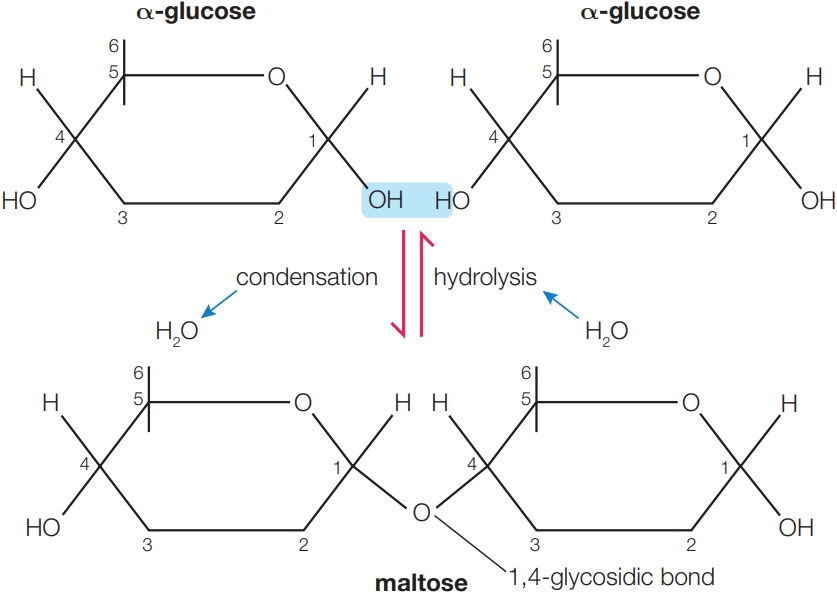
\includegraphics[scale=0.3]{Biology/1A/Images/1A-3-1.png}
                \caption{Glycosidic bonds are made by condensation reactions and broken down by hydrolysis.}
            \end{figure}
            \item \textbf{Exam Hint:} Avoid stating that energy is "created". Instead, describe how chemical energy from glucose
            is transferred to ATP molecules.
        \end{itemize}
    \end{itemize}
    \item \textbf{Properties of Polysaccharides}
    \begin{itemize}
        \item[1.] \textbf{Compact Structure:}
        \begin{itemize}
            \item Takes up little space within cells.
            \item Ideal for storage purposes.
        \end{itemize}
        \item[2.] \textbf{Insolubility:}
        \begin{itemize}
            \item Reduces \underline{osmotic effects} \footnote{\textbf{Osmotic effects:} Osmotic effects refer to the movement
            of water across a \underline{semipermeable membrane} \footnotemark[10] (半透膜) due to differences in solute
            concentration.} (渗透效应) in cells.
            \footnotetext[10]{\textbf{Semipermeable membrane:} It is a membrane that allows certain molecules to pass through
            while blocking others. It permits solvent molecules (such as water) to pass but prevents solute molecules from doing
            so. This property makes semipermeable membranes highly useful in various applications, such as
            \underline{desalination} (海水淡化), where water and salt in seawater are separated using a semipermeable membrane.}
            \item Does not affect water potential.
        \end{itemize} 
        \item[3.] \textbf{Chemical Inactivity:} Does not interfere with cellular reactions.
    \end{itemize}
    \item \textbf{Starch (Plant Energy Store)}
    \begin{itemize}
        \item Composed of $\alpha$-glucose units.
        \item Two main components:
        \begin{itemize}
            \item \textbf{\underline{Amylose} (直链淀粉):} Long, unbranched chains of $\alpha$-glucose units. Forms a compact
            spiral sturcture due to 1,4-glycosidic bonds.
            \item \textbf{\underline{Amylopectin} (支链淀粉):} Branched chains of $\alpha$-glucose units. Contains 1,4- and 1,6-
            glycosidic bonds, allowing rapid glucose release.
        \end{itemize}
        \begin{figure}[H]
            \centering
            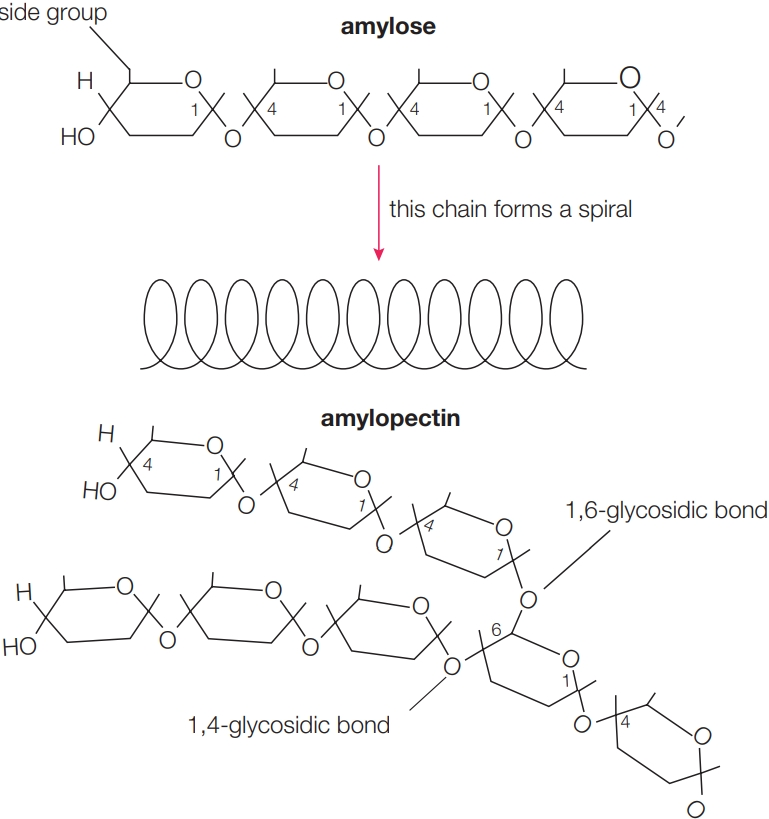
\includegraphics[scale=0.35]{Biology/1A/Images/1A-3-2.png}
            \caption{Amylose and amylopectin — a small difference in the position of the glycosidic bonds in the molecule makes
            a big difference to the properties of the compounds.}
        \end{figure}
        \item \textbf{Function:}
        \begin{itemize}
            \item Efficient energy storage in plants.
            \item Rapid glucose availability during high metabolic demands.
        \end{itemize}
        \item \textbf{Testing for Starch} If you add a few drops of reddish-brown iodine solution to a sample containing starch
        (whether it is a solid sample or a sample in solution), the iodine solution will turn blue-black.
        \begin{figure}[H]
            \centering
            \includegraphics[scale=1]{Biology/1A/Images/1A-3-5.bmp}
            \caption{The iodine test for starch.}
        \end{figure}
    \end{itemize}
    \item \textbf{Glycogen (Animal Energy Store)}
    \begin{itemize}
        \item Similar to amylopectin but more extensively branched.
        \item \textbf{Structure:}
        \begin{itemize}
            \item Contains many 1,6-glycosidic bonds, leading to multiple branches.
            \item Compact and can be rapidly hydrolyzed for energy.
        \end{itemize}
        \begin{figure}[H]
            \centering
            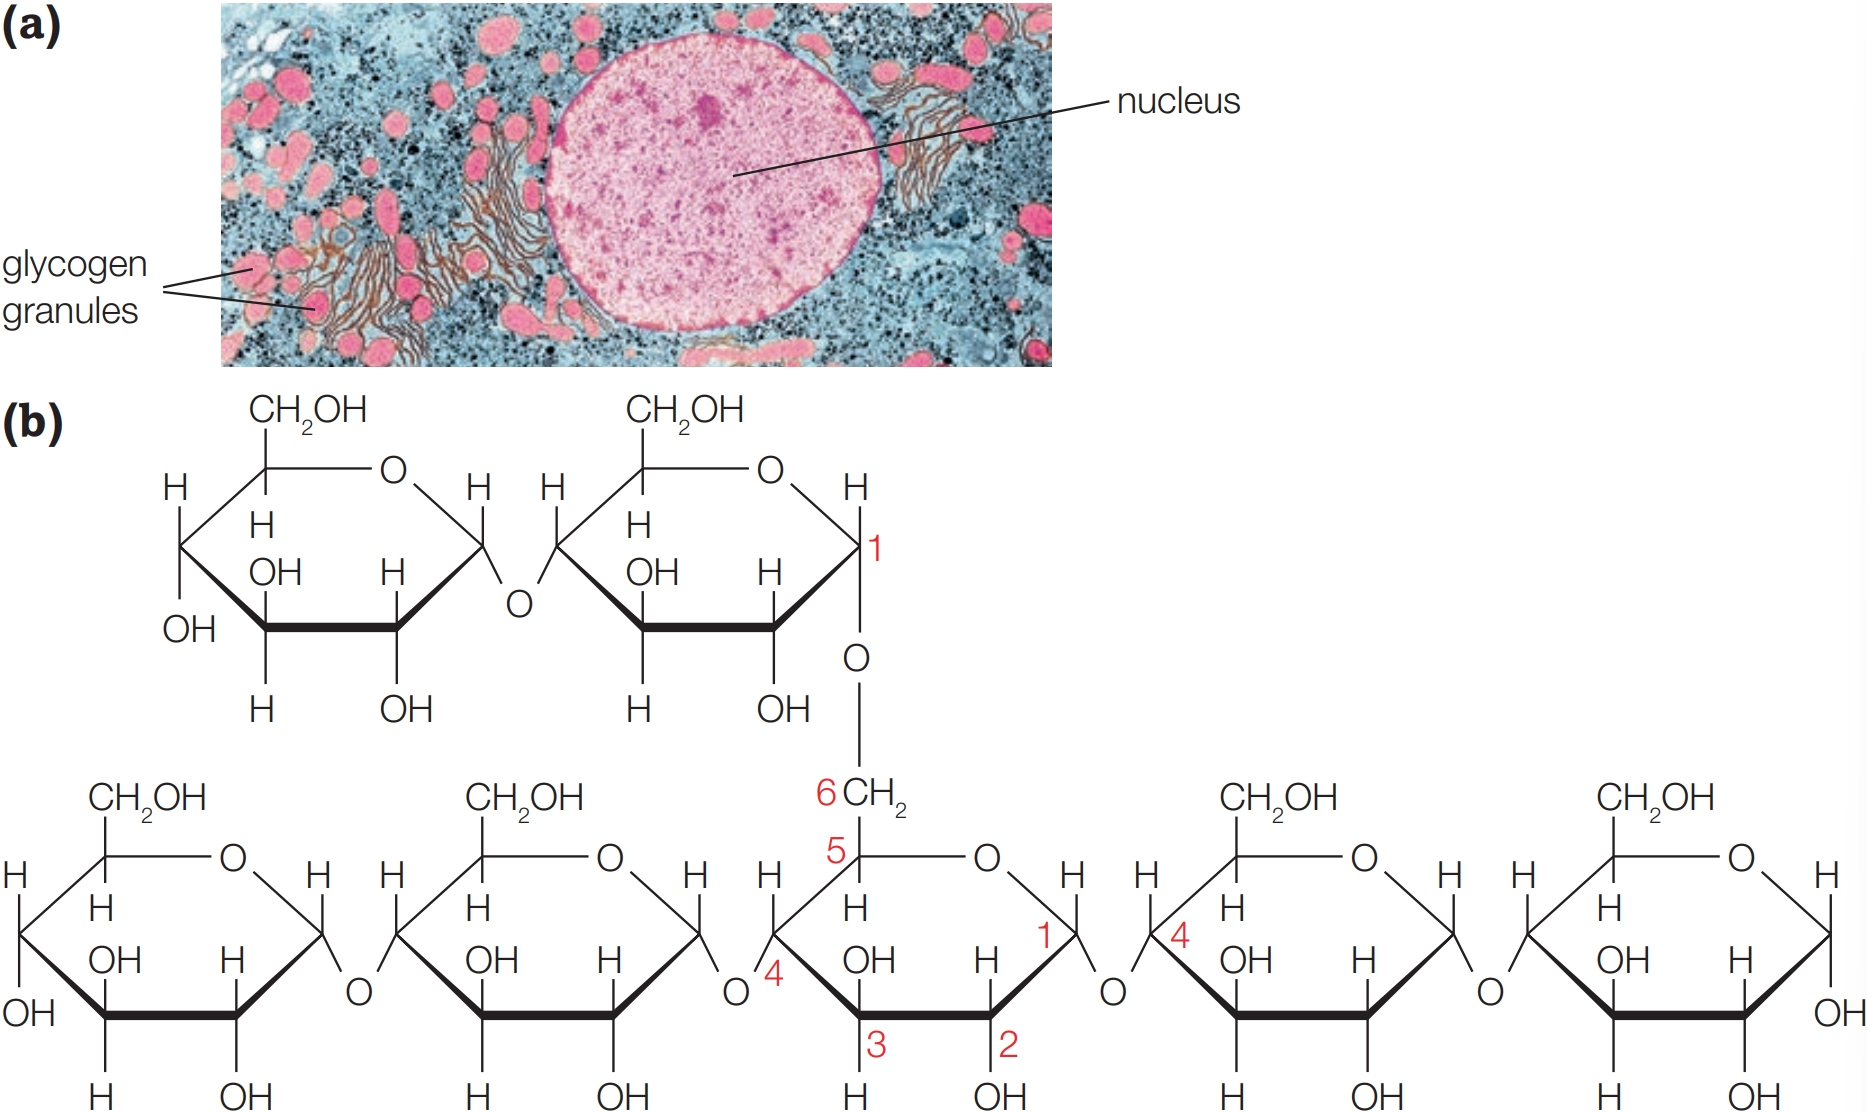
\includegraphics[scale=0.15]{Biology/1A/Images/1A-3-3.png}
            \caption{In \textbf{(a)} you can see liver cells full of small glycogen \underline{granules} (微粒), \underline{stained}
            (染色) pink in this \underline{micrograph} (显微照片). If your blood glucose levels are low, this glycogen store in
            your liver can be broken down to provide the glucose you need for cellular respiration. In \textbf{(b)} you can see the
            structure of glycogen with 1,4 and 1,6-glycosidic bonds.}
        \end{figure}
        \item \textbf{Function:}
        \begin{itemize}
            \item Found in the liver and muscle cells.
            \item Acts as a quick energy source for animal during high activity.
        \end{itemize}
        \begin{figure}[H]
            \centering
            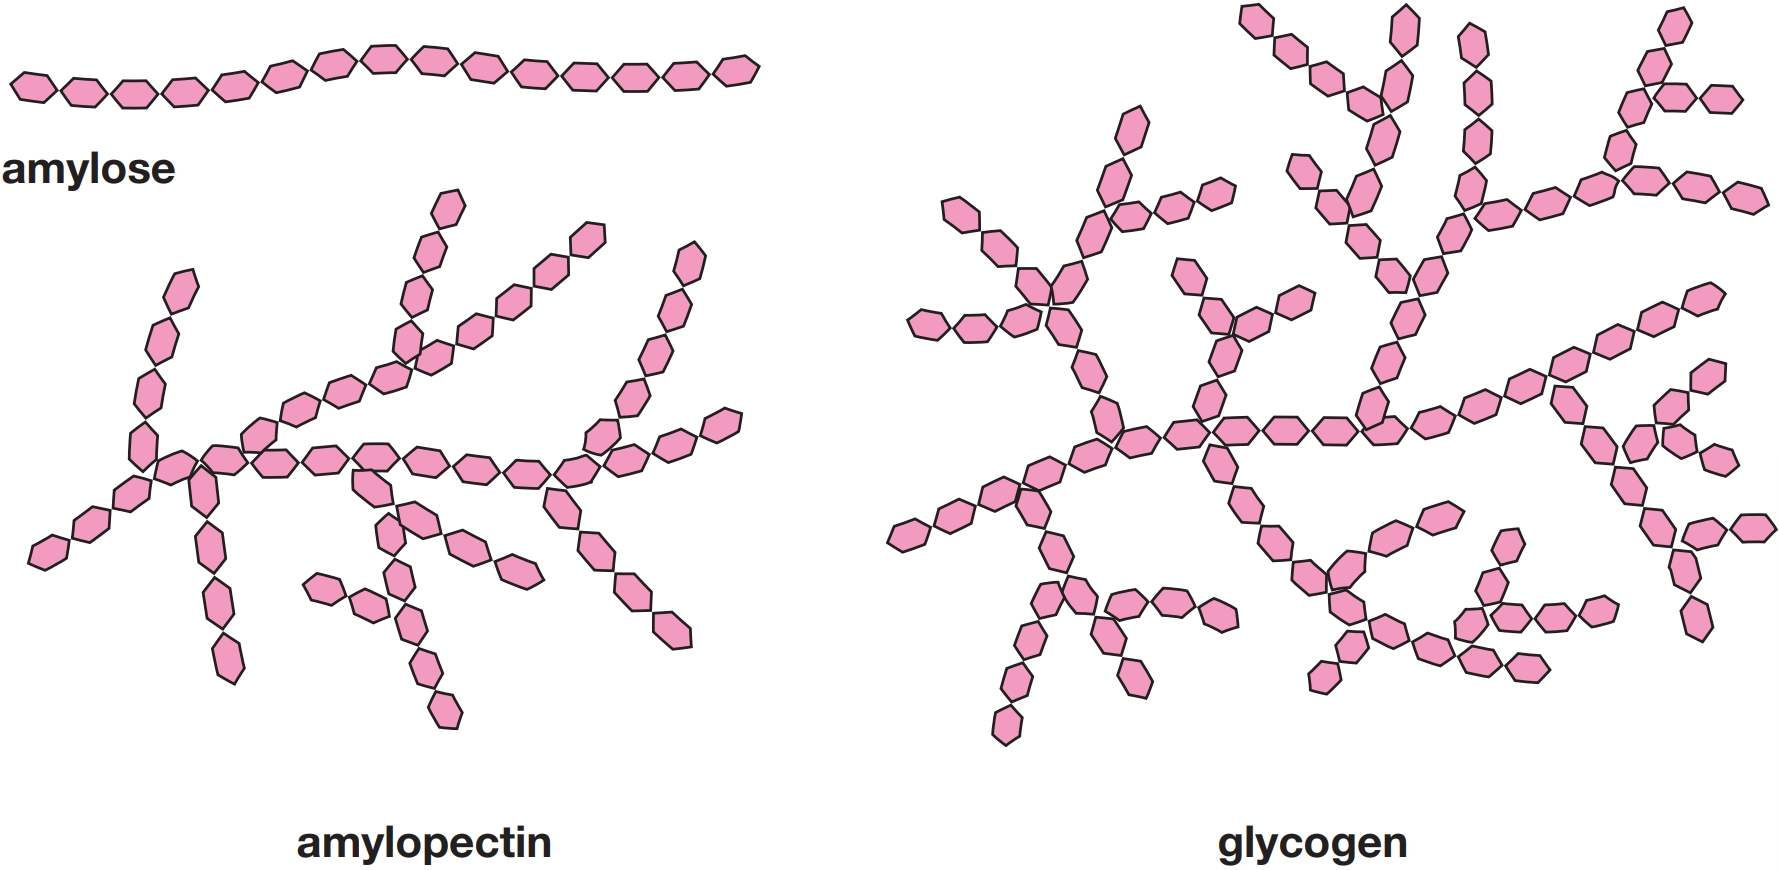
\includegraphics[scale=0.15]{Biology/1A/Images/1A-3-4.png}
            \caption{You can clearly see the many side branches which allow glycogen to be broken down so quickly when you
            compare amylose, amylopectin and glycogen.}
        \end{figure}
    \end{itemize}
\end{itemize}
